%%%%%   Capitulo 2 : Diseño de Especificaciones    %%%%%
\chapter{Definición de Especificaciones}

%%%%%   Revisión del Estado del Arte y de la Técnica    %%%%%
\section{Revisión del Estado del Arte y de la Técnica}
En la definición de las especificación necesarias para la máquina herramienta se procedió a una revisión dentro la literatura, las soluciones comerciales y las patentes creadas en base a esta temática. Por esto, este sección presentará lo encontrado en estos aspectos.

%%%%%   Estado del Arte    %%%%%
\subsection{Estado del Arte}
En las últimas décadas, la industria manufacturera ha sido beneficiada por las desarrollados alcanzados en la industria robótica, que han permitido una modernización de los procesos de manufactura, alcanzando altas prestaciones en cuanto a capacidad dinámica, rigidez, precisión \citep{serje2017parallel} así como en flexibilidad, eficiencia, bajo costo y seguridad \citep{yuan2018review,stipanvcic2012programming,vsvaco2014calibration}. La robótica no solo ha llamado la atención de la industria manufacturera, sino también a investigadores y académicos, esto es mostrado en la Figura \ref{fig:PublicacionesPorAnio}, donde se muestra el número de publicaciones con palabras clave “robótica” en Scopus \citep{yuan2018review}.

\begin{figure}[ht!]
    \centering
    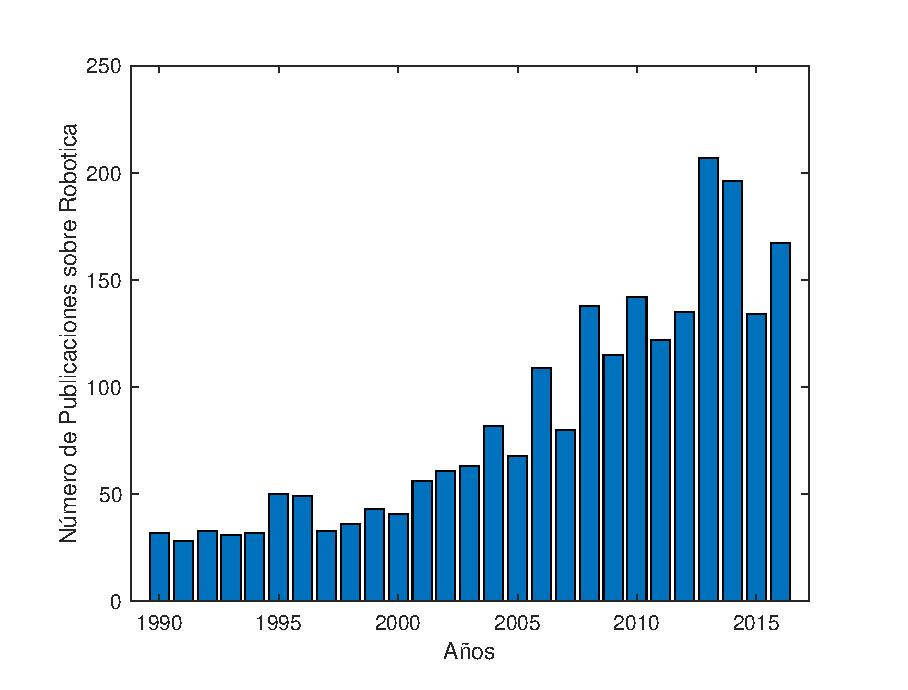
\includegraphics[width=0.7\textwidth]{Cap2_DisenoEspecificaciones/Figura/PublicacionesPorAnio.eps}
    \caption{Publicaciones por año}{Fuente:\citep{yuan2018review}}
    \label{fig:PublicacionesPorAnio}
\end{figure}

\subsubsection{Robot Herramienta Serial}

La industria de la robótica ha dejado a un lado los mecanismos convencionales para las máquinas herramientas, ver Figura \ref{fig:CartesianMachiningTool}, para utilizar una arquitectura serial, o de lazo abierto,  la cual consiste por una serie de eslabones unidos mediante juntas que permiten el movimiento relativo, ver Figura \ref{fig:MachiningSerialRobot}. Los primeras investigaciones sobre estos datan a inicios de los años 90’s, y desde entonces han sido intensamente investigado alrededor del mundo por su potencial de ser aplicado en distintos procesos de maquinado y manufactura \citep{chen2013robot}. Estas investigaciones abarcan temas como el diseño \citep{denkena2017design}, análisis de condición cinemática \citep{zargarbashi2012jacobian}, análisis de rigidez por su postura \citep{guo2015stiffness}, la utilización de redundancias [11], y el control de los mismo [12].

\begin{figure}[ht!]
    \centering
    \begin{subfigure}{0.45\textwidth}
        \centering
        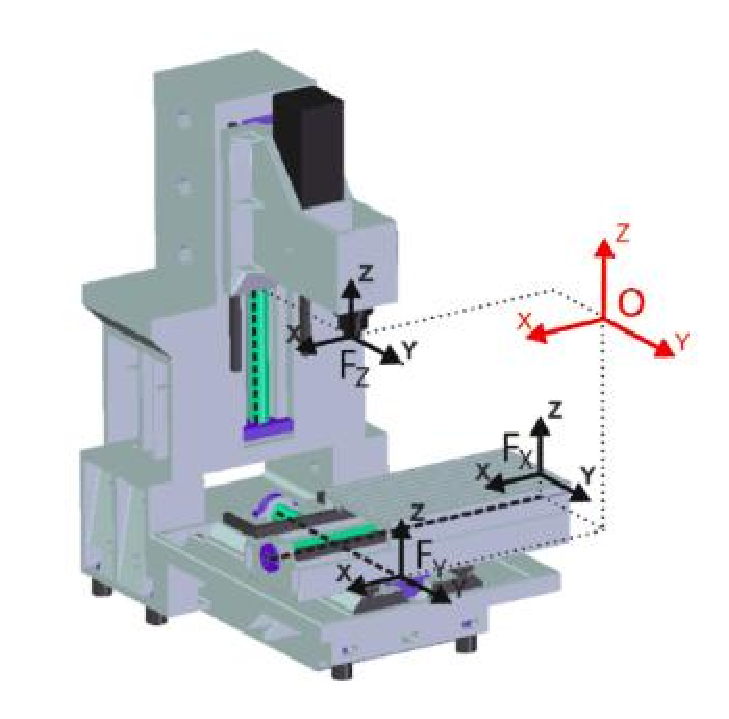
\includegraphics[width=0.8\linewidth]{Cap2_DisenoEspecificaciones/Figura/CartesianMachiningTool.pdf}
        \caption{Máquina Herramienta Cartesiana}{Fuente:\citep{szipka2018measurement}}
        \label{fig:CartesianMachiningTool}
    \end{subfigure}
     \begin{subfigure}{0.45\textwidth}
        \centering
        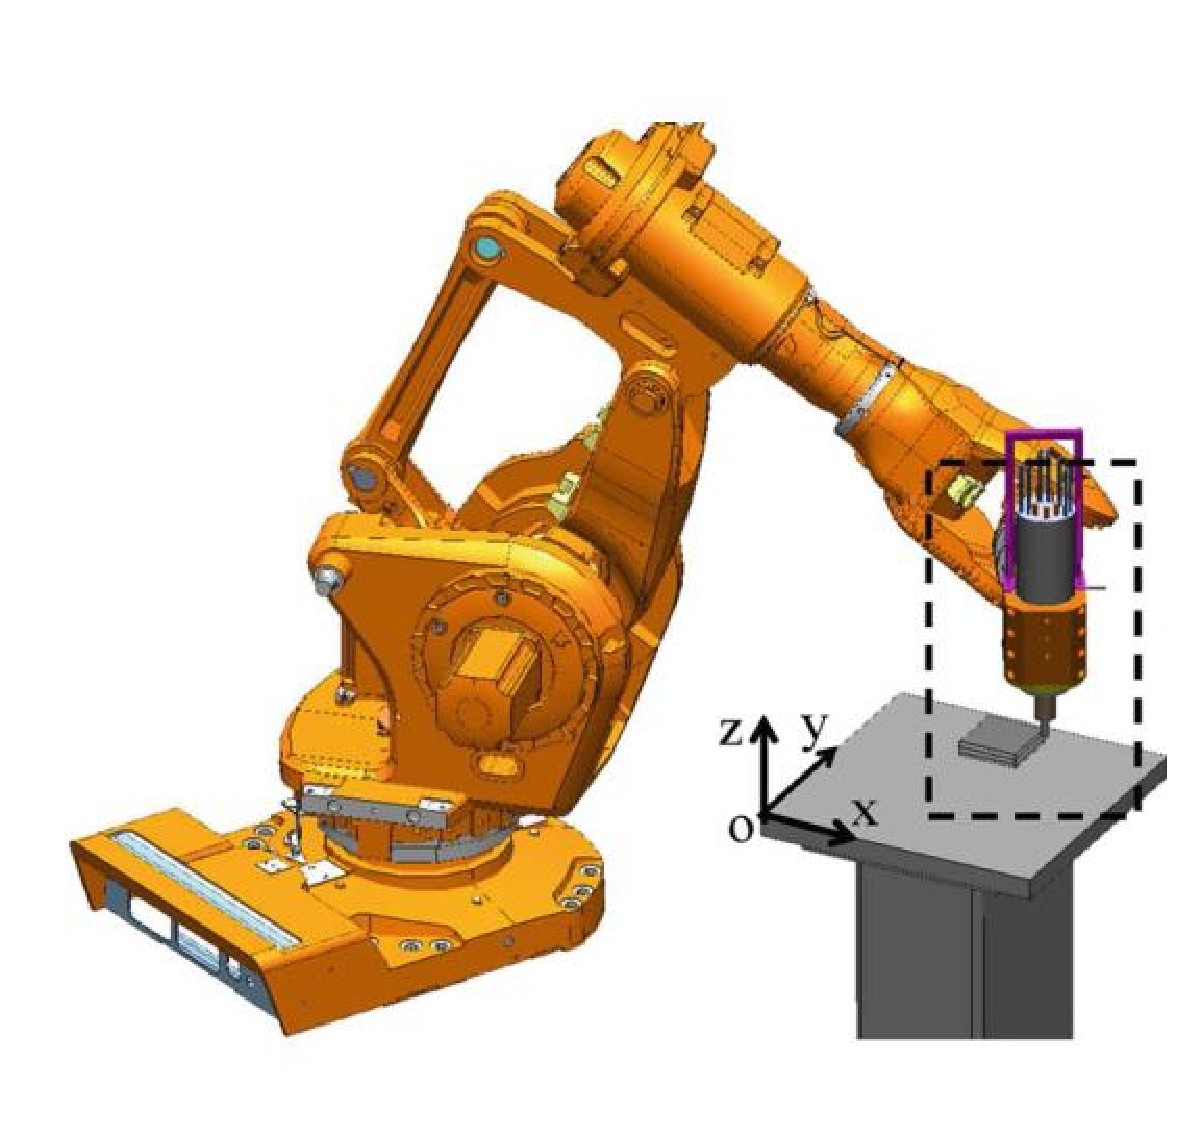
\includegraphics[width=0.8\linewidth]{Cap2_DisenoEspecificaciones/Figura/MachiningSerialRobot.pdf}
        \caption{Robot Herramienta Serial}{Fuente:\citep{mejri2016dynamic}}
        \label{fig:MachiningSerialRobot}
    \end{subfigure}
    \caption{Comparación de Maquina herramienta y Robot herramienta}
\end{figure}

En el diseño de robot seriales, \cite{denkena2017design} en su trabajo \enquote{Design and optimization of a machining robot} explica que para los robots seriales presentan una serie de debilidades y limitaciones frente a las máquinas herramientas convencionales. Siendo que la principal limitación es la rigidez del robot, debido a que es inferior si es comparada con las máquinas convencionales, y es importante en la precisión de la trayectoria a seguir así como en la productividad del mismo. Por esto, los autores antes de realizar el diseño detallado y optimización del robot, realizan una evaluación cinemática de los conceptos de máquinas, mostrando que esta desventaja puede ser eliminada utilizando una cinemática adaptada con menor número de juntas, ver Figura \ref{fig:07ConceptEvaluation}.

\begin{figure}[ht!]
    \centering
    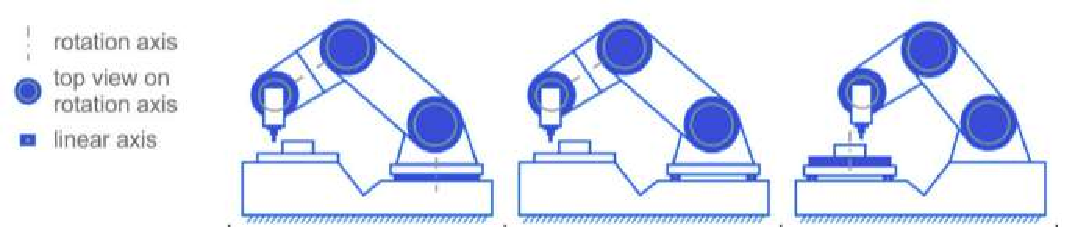
\includegraphics[width=0.8\textwidth]{Cap2_DisenoEspecificaciones/Figura/07ConceptEvaluation.pdf}
    \begin{tabular}[c]{p{0.2\textwidth} | m{0.2\textwidth} | m{0.2\textwidth} | m{0.2\textwidth} |}
         & Cinemática serial con solo juntas rotatorias & Cinemática serial guiada lineal & Cinemática serial con mesa lineal giratoria \\ \hline
        Rigidez & $\ominus$ & $\oplus$ &  $\oplus \oplus$ \\ \hline
        Modo Normal & $\ominus$ & $\oplus$ &  $\oplus \oplus$ \\ \hline
        Espacio & $\oplus$ & $\oplus$ & $\ominus$ \\ 
        de Instalación & & & \\ \hline
        Costo & $\oplus \oplus$ & $\oplus$ &  $\ominus \ominus$ \\ \hline
    \end{tabular}
    \caption{Conceptos de Robots seriales}{Fuente:\citep{denkena2017design}}
    \label{fig:07ConceptEvaluation}
\end{figure}

Por otra parte, en el análisis de condición cinemática, \cite{zargarbashi2012jacobian} en \enquote{The Jacobian condition number as a dexterity index in 6R machining robots} detalla sobre la utilización de un número de condición basado en el jacobiano como índice de desempeño. Teniendo en cuenta que este índice no tendría en cuenta los efectos dinámicos debido a las condiciones de trabajo durante el maquinado, siendo bajas velocidades, los efectos del husillo afectan la estructura y los altos modos de frecuencia del sistema. El número de condición trabaja teniendo en cuenta un pequeño error en las juntas, $\delta\dot\theta$, que produce un error en movimiento del efector, $\delta t$; recordando que las velocidades de estos elementos se relacionan a través de la matriz jacobiana, Ecuación \ref{Eq:IOVelocityEquation}, y que la inducción de este error en la posición, $\delta\theta$, afecta igualmente al jacobiano, $J\left(\theta + \delta\theta \right)$, sin embargo, puede ser aproximado de la siguiente manera $J\left(\theta + \delta\theta \right) \approx J\left(\theta\right)$. Por lo que los errores de velocidades pueden ser expresados por la Ecuación \ref{Eq:ErrorIOEquation}, simplificados de la forma Ecuación \ref{Eq:SimpleErrorIOEquation}, y en base a esto, el número de condición se obtiene relacionando la ecuación \ref{Eq:SimpleErrorIOEquation} con la ecuación \ref{Eq:IOVelocityEquation}, ver ecuaciones \ref{Eq:ConditionEquation} y \ref{Eq:ConditionExpression}. El número de condición manejaría valores entre $1$ y $\infty$, siendo que entre más pequeño el número de condición más uniforme será el cambio de las juntas sobre el efector.

\begin{subequations}
    \begin{eqnarray}
        \dot\theta = J^{-1}\left(\theta\right) t \label{Eq:IOVelocityEquation} \\
        \dot\theta + \delta\dot\theta = J^{-1}\left(\theta\right) \left(t + \delta t\right) \label{Eq:ErrorIOEquation} \\
        \delta\dot\theta = J^{-1}\left(\theta\right) \delta t \label{Eq:SimpleErrorIOEquation} \\
        \frac{\left\lVert \delta\dot\theta \right\rVert}{\left\lVert \dot\theta \right\rVert} \leq \kappa\left( J \right) \frac{\left\lVert \delta t \right\rVert}{\left\lVert t\right\rVert} \label{Eq:ConditionEquation} \\
        \kappa\left(J\right) = \left\lVert J\left(\theta\right) \right\rVert \cdot \left\lVert J^{-1}\left(\theta\right) \right\rVert \label{Eq:ConditionExpression}
    \end{eqnarray}
\end{subequations}

En el análisis de rigidez, el \cite{guo2015stiffness} y su artículo \enquote{Stiffness-oriented posture optimization in robotic machining applications} especifica un método optimización de postura de un robot serial que apunta a incrementar su rigidez, debido a que estos robots presentan múltiples soluciones para una posición del efector final \citep{zhu2013off}, como el ejemplo donde un robot de taladrado para un punto y dirección de un agujero no aplica una única pose, en la Figura \ref{fig:13OnePointTwoPoses} se muestra dos posibles poses del efector para taladrar un mismo agujero. Por eso, \cite{guo2015stiffness} mediante la utilización del modelo de rigidez del robot para seleccionar dentro de todas las poses posibles la que más óptima, es decir aquella que maximice la rigidez del sistema.

\begin{figure}[ht!]
    \centering
    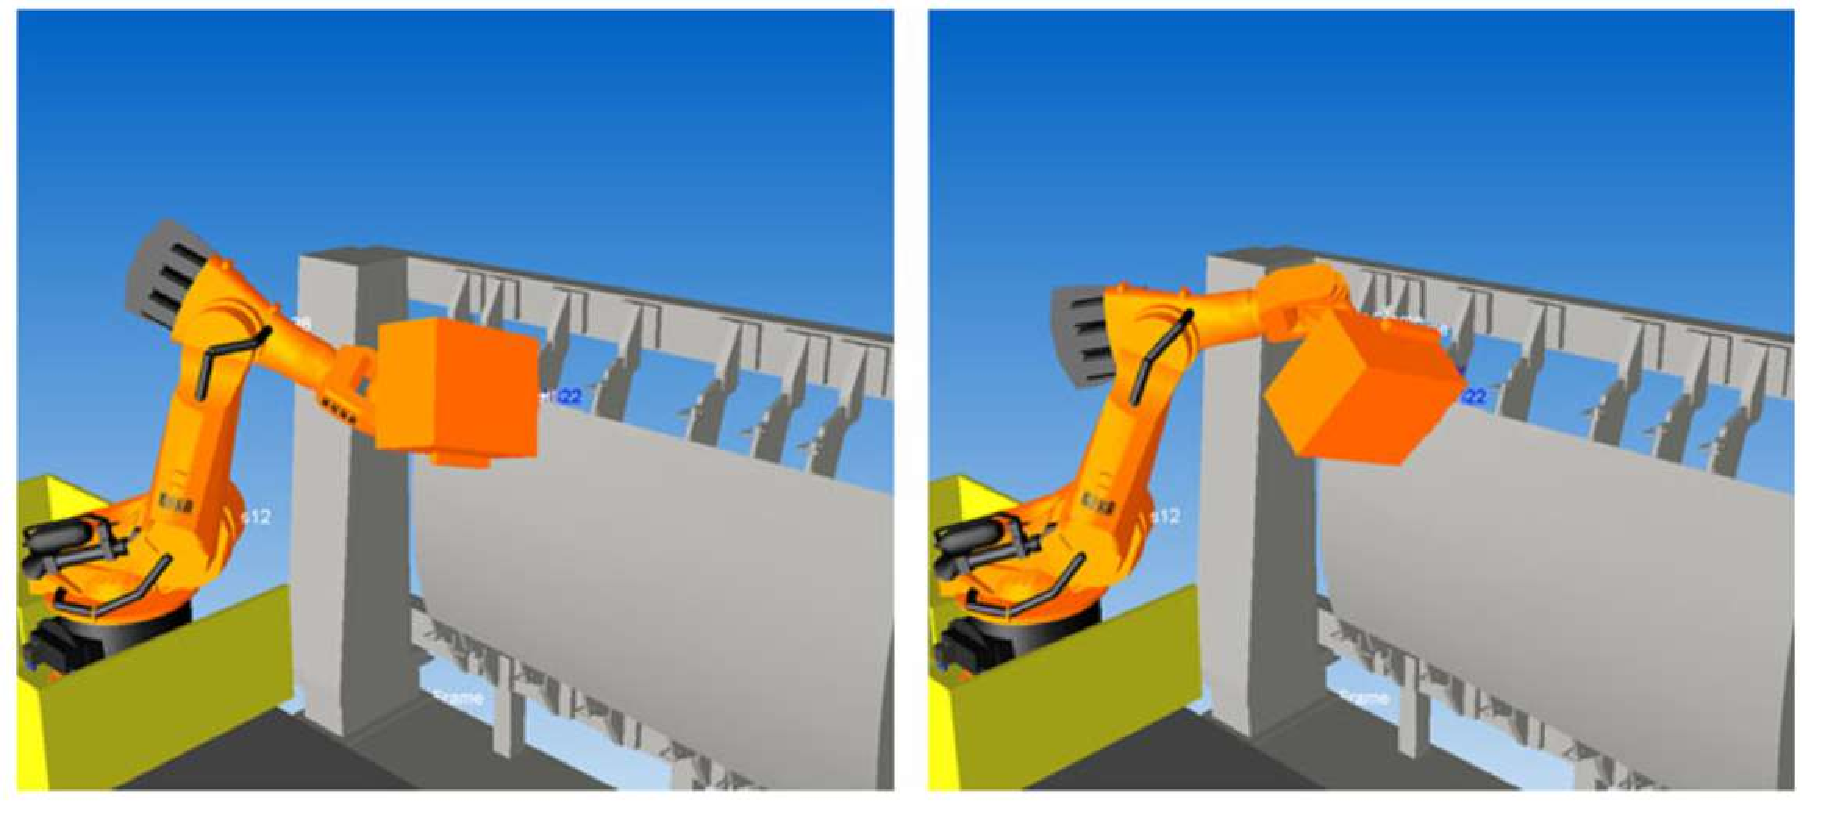
\includegraphics[width=0.7\textwidth]{Cap2_DisenoEspecificaciones/Figura/13OnePointTwoPoses.pdf}
    \caption{Multipes poses para un mismo punto}{Fuente:\citep{zhu2013off}}
    \label{fig:13OnePointTwoPoses}
\end{figure}

En la implementación de redundancias, \cite{subrin2013new} para su investigación \enquote{New redundant architectures in machining: serial and parallel robots} evalua el desempeño de una arquitectura redundante de robot serial, observando como la implementación de lazo cerrado mejora el rendimiento cinemático como el rendimiento de rigidez de un manipulador serial.

Para la calibración y control de los robots seriales, \cite{andres2011calibration} en trabajo \enquote{Calibration and control of a redundant robotic workcell for milling tasks} detalla el procedimiento para la sintonización de un manipulador serial ${KUKA}^{TM}$, en donde propone un método para la calibración de este dispositivo en el sitio, usando sensores láser de desplazamiento y con una restricción de plano de no contacto. Estos procedimientos son sencillos de implementar y los recomienda para la mayoría de los robots industriales por su rapidez en el sitio.

En breve de los robots seriales, son mecanismos con una cadena cinemática abierta, la cuál le otorga un amplio espacio de trabajo, múltiples posturas para un misma posición y sencillez en el control, pero del mismo modo, produce baja estabilidad y rigidez en el sistema.

\subsubsection{Robot Herramienta Paralelo}
La creciente demanda de productos con mejores especificaciones ha llevado a la industria de la fabricación a incrementar los requerimientos y el rendimiento de los robots industriales, exigiendo mayores niveles de precisión operacional, capacidad de trabajo, confiabilidad y ciclo de vida. Una tendencia para la satisfacción de estas demandas radica en la implementación de manipuladores paralelos, los cuales poseen un potencial de trabajo alto, resaltando características como su alta rigidez, alta precisión y alta capacidad de carga \citep{zhang2009parallel}, además de ciertas ventajas como forma isotrópica, espacio libre de singularidades, rendimiento kinostatico uniforme y reconfigurabilidad \citep{lin2015design,ur2009kinematic,ZENG2014648}; por esto han sido implementado en la rehabilitación de brazo, mover y poner, maquinado de precisión o simulador de braquiterapia \citep{briot2009pantopteron,cardou2010dimensional,hoppner2015two,martini2015static}.

Por esto en la literatura se estudia a los mecanismos paralelos desde el análisis de una configuración \citep{sarabandi2018reconfigurable}, análisis cinemático \citep{gallardo2014application}, análisis dinámico \citep{xu2017dynamic}, el diseño \citep{li2018design}, Optimización \citep{kelaiaia2012multiobjective} y el control \citep{cazalilla2016hybrid}.

En el análisis de configuración, está el caso de \cite{sarabandi2018reconfigurable}, quien en su artículo \enquote{A Reconfigurable Asymmetric 3-UPU Parallel Robot} analiza la arquitectura UPU, \textit{Universal - Prismática - Universal}, por la posibilidad que tiene un mecanismo de tres brazos con esta arquitectura de presentar un movimiento puramente traslacional o puramente rotacional según su modo de ensamble. Esta configuración fue previamente estudiada por \cite{di1998translational}, quien determinó cuales son las condiciones que deben cumplir las universales, más específicamente el par de revolutas que la conforman, para producir movimientos de traslación; por otro lado, \cite{karouia2000three} estudio las condiciones constructivas que permiten un movimiento completamente rotacional en la plataforma. Sin embargo, el mecanismo presenta una sensibilidad a errores y zonas de su espacio de trabajo donde tiene un movimiento mixto,   traslación – rotación, y es por esto que los autores introducen una configuración asimétrica que permita prevenir estos inconvenientes de la arquitectura.

\begin{figure}
    \centering
    \begin{subfigure}{0.45\textwidth}
        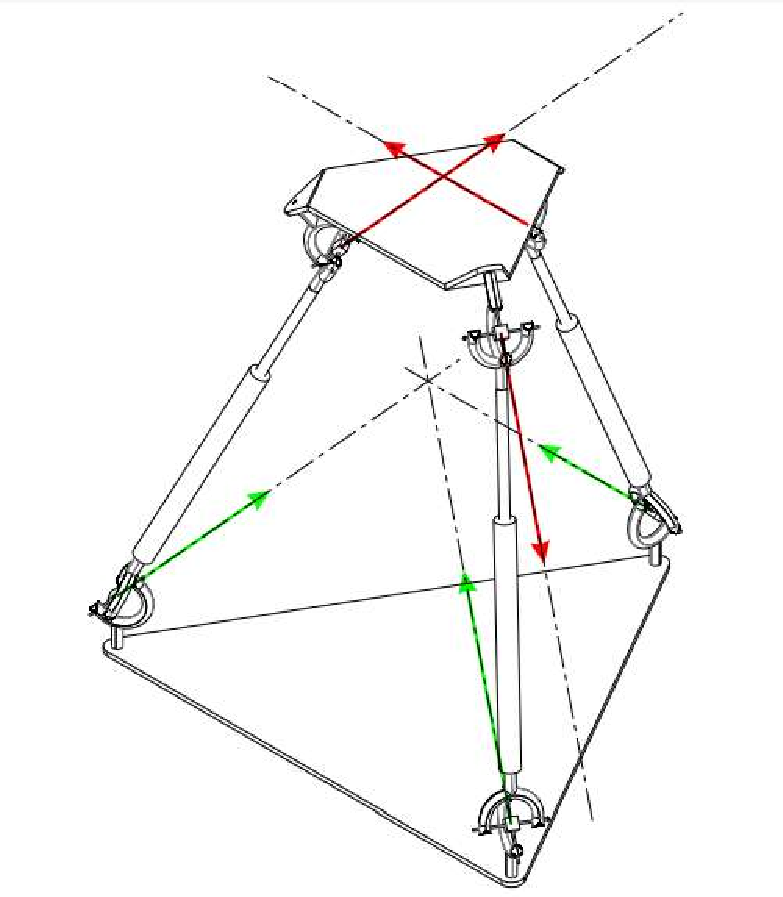
\includegraphics[width=0.9\linewidth]{Cap2_DisenoEspecificaciones/Figura/Sarabandi2018-01.pdf}
        \caption{Mecanismo Traslacional}
        \label{fig:Sarabandi2018-01}
    \end{subfigure}
    \begin{subfigure}{0.45\textwidth}
        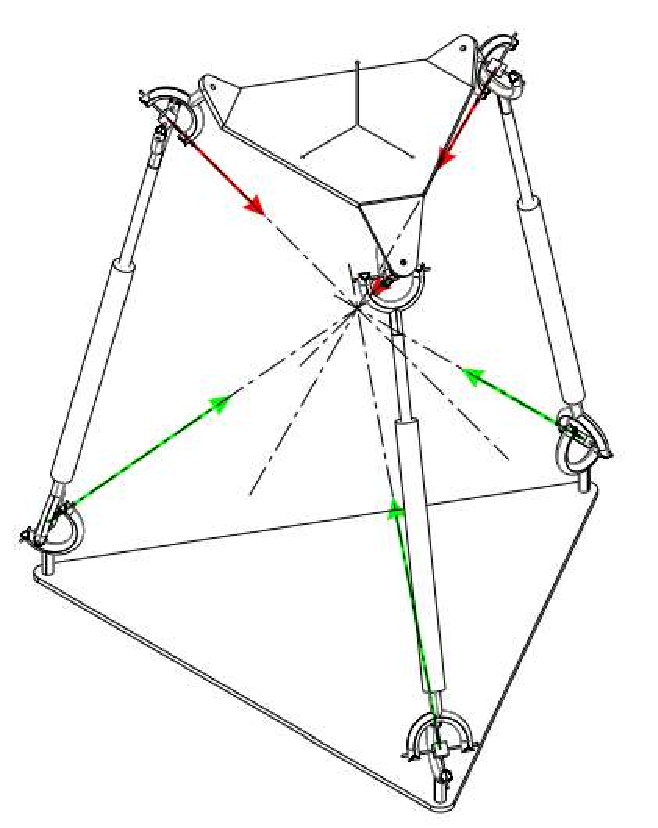
\includegraphics[width=0.8\linewidth]{Cap2_DisenoEspecificaciones/Figura/Sarabandi2018-02.pdf}
        \caption{Mecanismo Rotacional}
        \label{fig:Sarabandi2018-02}
    \end{subfigure}
    \caption{Arquitectura propuesta por \cite{sarabandi2018reconfigurable}}
    \label{fig:Sarabandi2018}
\end{figure}

En el análisis cinemático, \cite{gallardo2014application} en su trabajo \enquote{An application of screw theory to the kinematic analysis of a Delta-type robot} detalla los pasos de un análisis cinemático para un mecanismo tipo delta, ver Figura \ref{fig:Gallardo2014}, explicando el método por \citep{pierrot1990delta} para resolver el problema de cinemática inversa de este; para después realizar el análisis de velocidades aplicando teoría de tornillo, un recurso matemático que hace uso de las coordenadas de Plücker para simbolizar el estado de movimiento de cada revoluta además de la forma de Klein de la algebra de Lie para calcular las velocidades; por último, el análisis de aceleración aplica la misma teoría; los resultados son verificados con un software de simulación llamado ADAMS.

\begin{figure}[htb!]
    \centering
    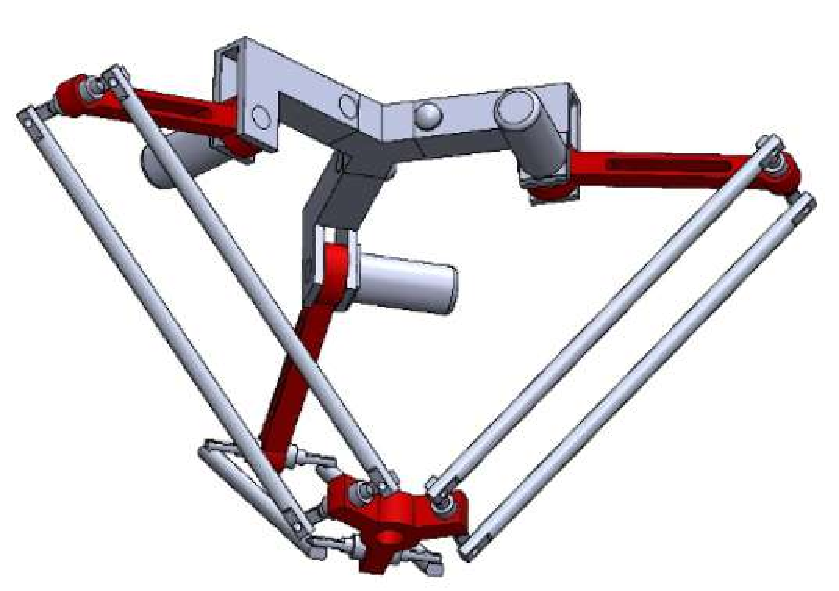
\includegraphics[width=0.5\textwidth]{Cap2_DisenoEspecificaciones/Figura/Gallardo2014.pdf}
    \caption{Robot delta simulado en ADAMS}{Fuente: \citep{gallardo2014application}}
    \label{fig:Gallardo2014}
\end{figure}

En el análisis dinámico, \cite{xu2017dynamic} explica, en \enquote{Dynamic analysis of a linear Delta robot in hybrid polishing machine based on the principle of virtual work}, un método llamado trabajo virtual para resolver el análisis dinámico de un robot delta lineal, ver Figura \ref{fig:Xu2017}; dicho método apunta a resolver las fuerzas motrices de las juntas prismáticas, teniendo en cuenta las fuerzas y momentos inerciales de cada cuerpo móvil alrededor del punto de pivote. Por otro lado, esta metodología recibe su nombre debido a que se supone un desplazamiento virtual, interrelacionando los desplazamientos de cada cuerpo con las entradas a través de matrices jacobianas, con esto se calcula los trabajos realizados por todas las fuerzas externas del mecanismo, y por último, se determinan las fuerzas de los actuadores.

\begin{figure}[hbt!]
    \centering
    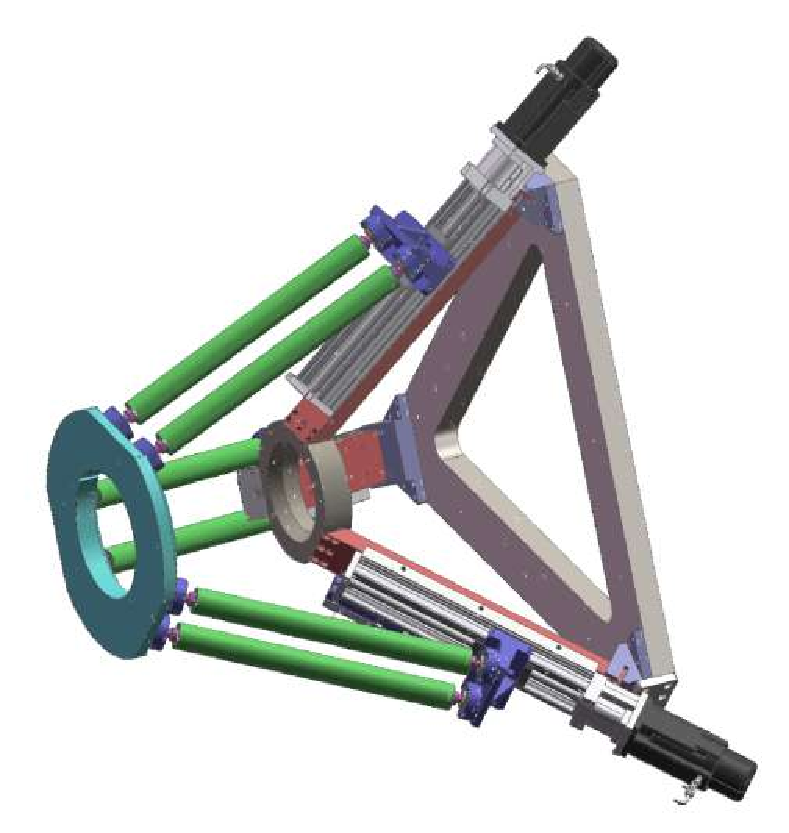
\includegraphics[width=0.4\textwidth]{Cap2_DisenoEspecificaciones/Figura/Xu2017.pdf}
    \caption{Modelo 3D del robot paralelo}{Fuente: \citep{xu2017dynamic}}
    \label{fig:Xu2017}
\end{figure}

En el diseño, \cite{li2018design} trabaja el diseño de un robot paralelo con configuración 3-CPS, esto lo hace en el artículo \enquote{The design of a 3-CPS parallel robot for maximum dexterity}. En la primera etapa del diseño se selecciona la arquitectura con la que se va a trabajar, especificando sus ventajas y desventajas, para su caso escogieron los SDelta, ver Figura \ref{fig:Li2018}, debido a que son robots paralelos con 6 grados de libertad, esto implementando 3 brazos, de ahí que eviten interferencia entre los brazos, así como baja carga inercial. Además todos sus motores están ubicados en la base. Luego de esto, el procedimiento de diseño continúa con los análisis cinemáticos y cinéticos, determinando la cinemática inversa o la directa, un análisis de singularidades y por último, un análisis de fuerzas. Esto es hecho para mirar el comportamiento del mecanismo ante una medidas determinadas. El diseño prosigue con una optimización dimensional, la cual se hace es llevada a cabo midiendo un índice de desempeño. Este índice o conjunto de índice son escogidos en función de los requerimientos de la aplicación.

\begin{figure}[hbt!]
    \centering
    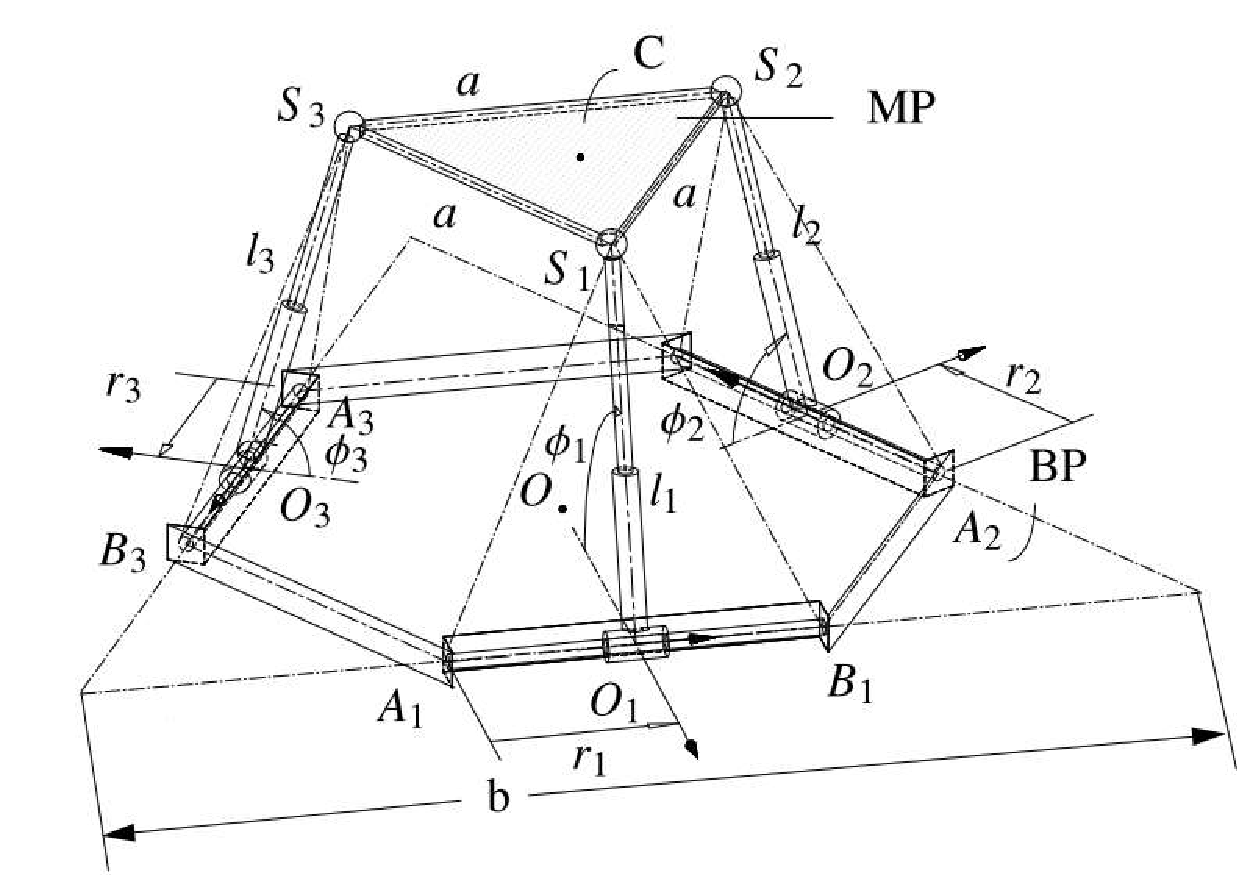
\includegraphics[width=0.5\textwidth]{Cap2_DisenoEspecificaciones/Figura/Li2018.pdf}
    \caption{Arquitectura SDelta}{Fuente: \citep{li2018design}}
    \label{fig:Li2018}
\end{figure}

En la Optimización, \cite{kelaiaia2012multiobjective} en su trabajo \enquote{Multiobjective optimization of a linear Delta parallel robot} muestra como la síntesis dimensional es vital para el buen diseño de un robot paralelo. Propone una metodología para este problema, ver Figura \ref{fig:Kelaiaia2012}, el cual es expresado en términos de una optimización multiobjetivos teniendo en cuenta varios criterios de rendimiento. Dichos criterios de evaluación miden el rendimiento del espacio de trabajo, la rigidez, así como el comportamiento cinemático y dinámico. Para llevar a cabo la optimización utilizan un algoritmo genético SPEA-II, configurado con 200 miembros de la población, 200 generaciones, 90\% de probabilidad de cruzamiento y probabilidad de mutación del 10\%.

\begin{figure}[hbt!]
    \centering
    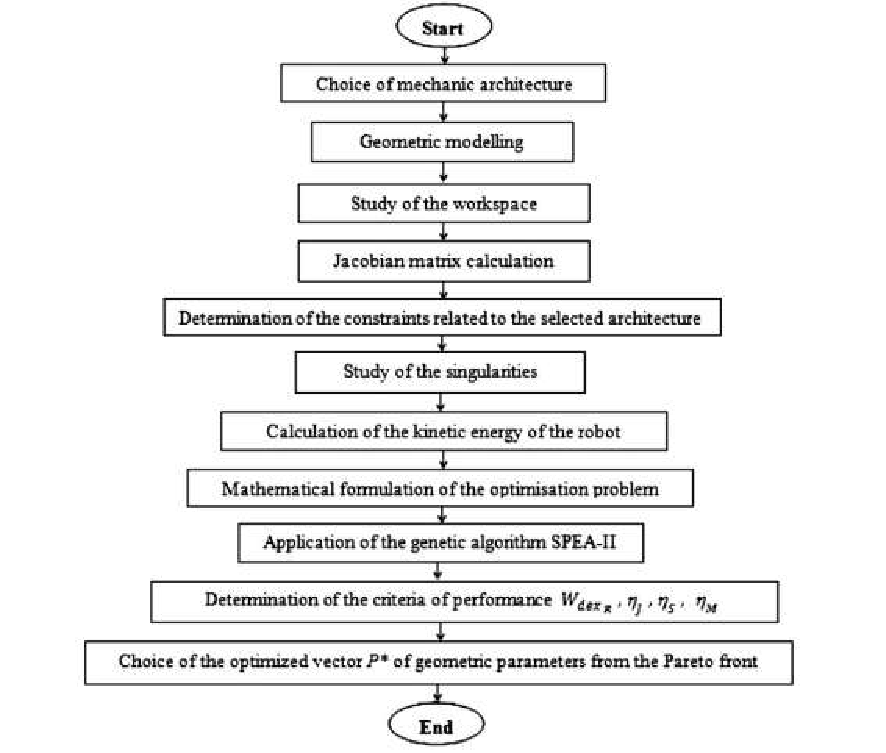
\includegraphics[width=0.5\textwidth]{Cap2_DisenoEspecificaciones/Figura/Kelaiaia2012.pdf}
    \caption{Metodología propuesta}{Fuente: \citep{kelaiaia2012multiobjective}}
    \label{fig:Kelaiaia2012}
\end{figure}

En breve, los robots paralelos presentan una serie de ventajas cinemáticas y dinámicas, comparados con las otras dos tecnologías. Para aprovechar estas ventajas en la etapa de diseño, se deben analizar desde la arquitectura, pasando por cada uno de los análisis cinemáticos y cinéticos, así como otros necesarios para los criterios de la aplicación, hasta la parte de la síntesis dimensional del mecanismo.

\begin{center}
    \begin{longtable}{>{\columncolor[gray]{0.85}} p{0.3\textwidth} p{0.3\textwidth} p{0.3\textwidth} }
        \rowcolor[gray]{0.85}
         & \centering \textbf{Comparativo de las arquitectura}  & \\   \hline
        \textbf{Caracteristicas} & \textbf{Serial} & \textbf{Paralela} \\
        \endfirsthead \hline
        \textbf{Caracteristicas} & \textbf{Serial} & \textbf{Paralela} \\ \hline \endhead \hline 
        Cinemática & \Large $\star\star\star\star\star$ & \Large $\star\star$ \\
         & Simple & Compleja \\ \hline
        Capacidad Dinamica & \Large $\star\star\star$ & \Large $\star\star\star\star\star$ \\
         & Limitada & Elevada \\ \hline
        Rigidez & \Large $\star\star$ & \Large $\star\star\star\star\star$ \\
         & Pobre & Elevado \\ \hline
        Destreza & \Large $\star\star\star\star\star$ & \Large $\star\star\star$ \\
         & Excelente & Alto \\ \hline
        Control & \Large $\star\star\star\star\star$ & \Large $\star\star$ \\
         & Simple & Compleja \\ \hline
        Modularidad & \Large $\star\star\star$ & \Large $\star\star\star\star\star$ \\
         & Alto & Excelente \\ \hline
        \caption{Resumen del estado de los robots}
        \label{table:ResumenEstadodelArteMecanismo}
    \end{longtable}
\end{center}

%%%%%   Estado de la Técnica    %%%%%
\subsection{Estado de la Técnica}

En la industria actual existe una amplia oferta de equipos para llevar a cabo procesos de fabricación de piezas de alta calidad como el maquinado. En cuanto al proceso de fresado existen 3 tipos de soluciones comerciales actuales muy competitivas en el mercado.

\begin{longtable}[c]{m{0.5\textwidth} m{0.05\textwidth} m{0.35\textwidth}}
    \hline \rowcolor[gray]{0.9} \textbf{EUROPA} & & \\ \hline
    \textbf{Empresas} & \textbf{Ejes} & \textbf{Aplicación} \\
    Demaurex/Delta          & 3 & Manipulador \\
    PKMtricept SL           & 5 & Maquinado, Ensamblaje \\
    %Geodetics               & 6 & Maquinado \\
    Carl Zeiss Jena, Physik Instrumente         & 6 & Posicionamiento \\
    %Physik, Instrumente     & 6 & Posicionamiento \\
    %CMW                     & 6 & Maquinado \\
    Lapic Company           & 6 & Medición de coordenadas \\
    Fooke (Triomax)         & 3 & Corte agua/láser \\
    Urane SX (Renault)      & 3 & Taladrado de alta velocidad \\
    %Simparalell (Simplex), Starrag Group (Ecospeed 20210), Teknodrom (XT 1100S)   & 5 & Maquinado \\
    %Starrag Group (Ecospeed 20210) & 5 & Maquinado \\
    %Teknodrom (XT 1100S)    & 5 & Maquinado \\
    \textbf{Universidad-empresa} & & \\
    WZL Aachen – Ingersoll  & 6 & Maquinado \\
    %FhG Chemnitz – Mikromat & 5 & Maquinado \\
    IfW Stuttgart – INA (Hexact) & 5 & Maquinado \\
    ETH Zurich – Mikron (Triaglide) & 3 & Maquinado \\
    \textbf{Universidades} & & \\
    ISW Stuttgart (Linapod) & 3 & Maquinado \\
    IWF – Hannover          & 3 & Maquinado láser\\
    ETH Zurich (Hexaglide), ITIA – CNR (Acrobat)  & 6 & Maquinado \\
    %ITIA – CNR (Acrobat)    & 6 & Maquinado \\
    \hline \rowcolor[gray]{0.9} \textbf{ESTADOS UNIDOS} & & \\ \hline
    \textbf{Empresa} & & \\
    Tornado 2000 (Hexel), Rotapod (Hexel), Variax (Giddings and Lewis)    & 6 & Maquinado \\
    %Rotapod (Hexel)         & 6 & Maquinado \\
    %Variax (Giddings and Lewis) & 6 & Maquinado \\
    \hline \rowcolor[gray]{0.9} \textbf{ASIA} & & \\ \hline
    \textbf{Universidad-empresa} & & \\
    Eclipse – Universidad de Seul, Leadwell (X-700R), Okuma, HexaM & 6 & Maquinado \\
    %Leadwell (X-700R)       & 6 & Maquinado \\
    %Okuma                   & 6 & Maquinado \\
    %HexaM                   & 6 & Maquinado \\
    Honda Engineering       & 3 & Maquinado \\
    Fanuc Robotics (F-200i) & 6 & Soldadura \\ \hline
    \caption{Empresas fabricantes de maquinas herramientas}{Fuente: \citep{serje2017parallel}}
\end{longtable}
En los últimos años han surgido diversas iniciativas investigativas y propuestas sobre la aplicación de robots con arquitecturas paralelas como solución a ciertas limitaciones de las máquinas herramientas seriales. Algunos de estos diseños se han logrado comercializar ofreciendo mejoras en las capacidades dinámicas y rigidez de las máquinas herramientas entrando a la competencia de la industria de la fabricación y a su vez presentando nuevos retos de diseño y control. En la siguiente tabla se presentan algunas de las maquinas herramientas fabricadas hasta la fecha y las aplicaciones que estas han tenido.

~



\begin{longtable}{|>{\columncolor[gray]{0.85}}p{0.16\textwidth}|p{0.16\textwidth}|p{0.16\textwidth}|p{0.12\textwidth}|p{0.18\textwidth}|p{0.1\textwidth}|}
    \hline \rowcolor[gray]{0.85}
    \textbf{Fabricante} & \textbf{Modelo} & \textbf{Arquitectura} & \textbf{Velocidad} $\left[ m/min \right]$ & \textbf{ET} $\left[ mm \right]$  & \textbf{ET/VM} $\left[ \% \right]$ \\ \hline \endhead
    
    CharlyRobot  & Charly4U     & Paralela & 6     & 310x220x160   & --\\\cline{1-6}
    Chiron       & V-Concept    & Hibrida  & 120   & 450x300x300   & 2.77\\ \cline{1-6}
    DMG mori     & CMX600 V     & Cartesiana & 30  & 600x560x510   & 1.07\\ 
                 & CMX800 V     & Cartesiana & 30  & 800x560x510   & 0.82\\ 
                 & CMX1100 V    & Cartesiana & 30  & 1100x560x510  & 0.95\\\cline{1-6}
    Fatronik     & Ulyses       & Paralela & 50    & 500x500x500   & --\\ \cline{1-6}
    Hass         & VF-1         & Serial   & 16.5  & 508x406x508   & 0.63\\ 
    Automation   & Minimill2    & Serial   & 15.2  & 508x406x356   & 0.55\\ 
                 & OM-1A        & Serial   & 19.2  & 203x203x305   & 0.52\\\cline{1-6}
    Heckert      & SKM400       & Paralela & 100   & 630x630x630   & --\\ \cline{1-6}
    Hitachi Seiki & PA35II      & Paralela & 100   & 350x350x200   & --\\ \cline{1-6}
    Honda        & HVS500       & Hibrida  & 60    & 650x500x400   & --\\ \cline{1-6}
    HullerHille  & Specht-      & Hibrida  & 120   & 630x630x750   & --\\ 
                 & Xperimental  &          &       &               &   \\ \cline{1-6}
    Index        & V100         & Paralela & 50    & 280x280x145   & 0.09\\ \cline{1-6}
    ISWstuttgart & Linapod      & Paralela & 45    & 400x400x400   & 0.46\\ \cline{1-6}
    IRCCyN       & Orthoglide   & Paralela & 100   & 200x200x200   & 0.46\\ \cline{1-6}
    JSWAY        & JDV850       & Paralela & 10    & 800x500x500   & 1.04\\ \cline{1-6}
    Krauseco     & QuickStep    & Paralela & 80    & 630x630x500   & --\\ 
     Mauser      & HS500        &          &       &               &    \\ \cline{1-6}
    Leadwell CNC & V-20i        & Cartesiana &       & 510x350x400   & --\\
    Machines     & V-30         & Cartesiana &       & 600x400x300   & --\\ \cline{1-6}
    Light        & Spectra      & serial   & 0.76  & 216x114x140   & 1.73\\
    Machines Corp & light200    &          &       &               &   \\ \cline{1-6}
    Mazak        & VC-300A      & Paralela & 24    & 350x300x305   & 0.50\\ 
                 & VC-500C      & Paralela & 30    & 500x1000x510  & 0.07\\ 
                 & VC-500A/2PC  & Paralela & 30    & 505x505x510   & 4.70\\ \cline{1-6}
    Mikron       & Triaglide    & Paralela &       & 170x120x250   & 0.16\\ \cline{1-6}
    OKuma        & MB-46V       & Paralela & 32    & 500x460x460   & 0.75\\ 
                 & MB-500H      & Paralela & 60    & 500x500x460   & 0.28\\ \cline{1-6}
    Sharp        & LMV-50       & Paralela &       & 812,279x127   & 4.25\\ 
                 & TMV          & Paralela &       & 711x381x127   & 2.14\\ 
                 & LMV          & Paralela &       & 635x279x127   & 3.83\\\cline{1-6}
   Techno Inc    & RG5950       & Paralela & 20.32 & 1500x1300x254 & 6.58\\ \cline{1-6} 
   Mikron        & Triaglide    & Paralela &       & 170x120x250   & 0.16\\ \cline{1-6}
   University    & LOLA         & Paralela & 10    & 120x100x35    & 0.35\\ 
   of Belgrade   &              &          &       &               &   \\ \cline{1-6}
   WZL Aachen    & DynaM        & Hibrida  & 90    & 630x630x500   & 2.21\\ \cline{1-6}
                 
                            
    \caption{ Máquinas Fresadoras de 3 ejes actuales}{Fuente: Elaboración propia}
\end{longtable}
La tabla anterior realiza una comparativa de algunas especificaciones de fresadoras de 3 ejes abarcando una amplia gama de capacidades, distintos fabricantes y arquitecturas. Como resultado de esta encontramos velocidades lineales promedio de 45m/min para espacios de trabajo de 550x450x370 mm con una compacidad de la máquina de 1.5\%. La tabla es resultado de elaboración propia con adaptaciones de \cite{serje2017parallel}.


%\begin{figure}[ht!]
%    \centering
%    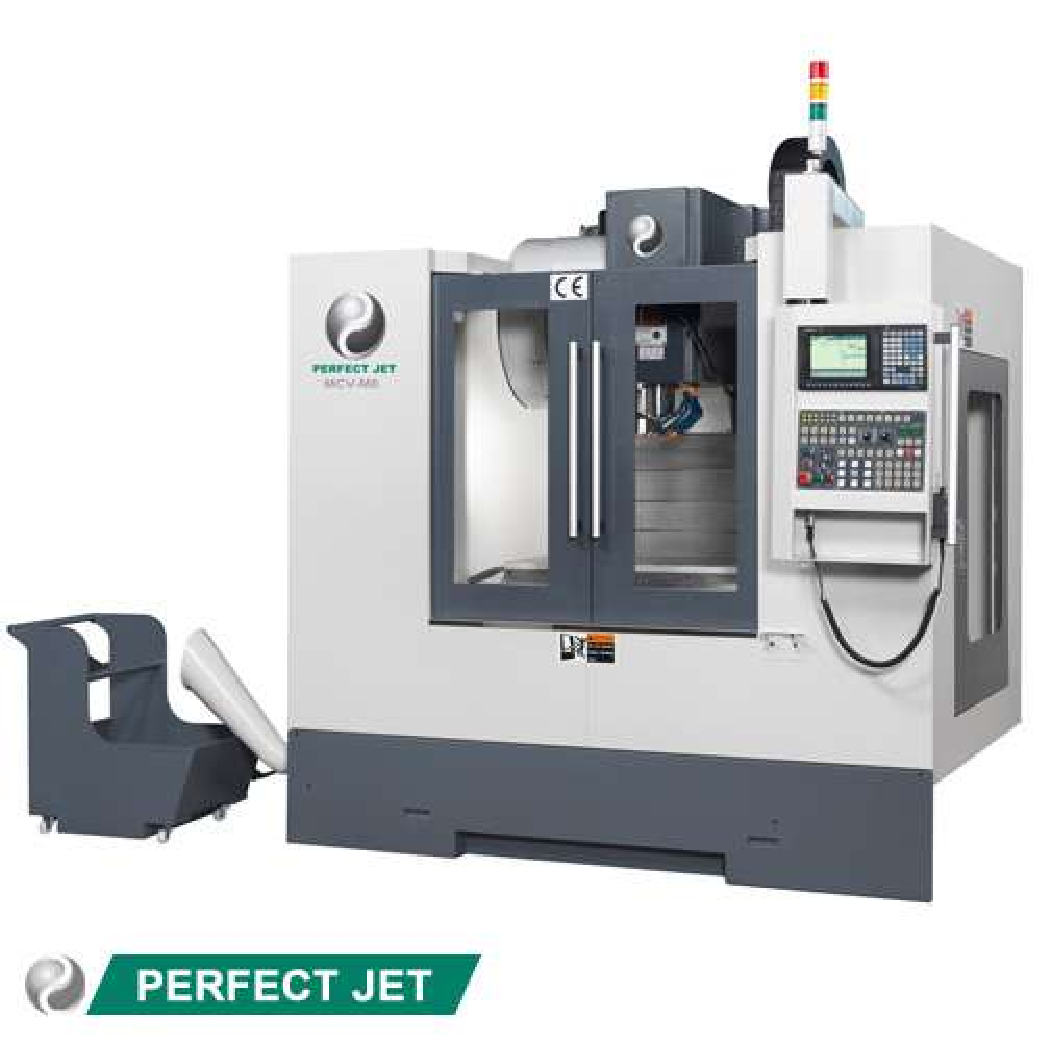
\includegraphics[width = 0.5\textwidth]{Cap2_DisenoEspecificaciones/Figura/Perfect-Jet_MCV-M8.pdf}
%    \caption{Máquina Herramienta de Perfect-jet}
%    \label{fig:Perfect_jet-MCV-M8}
%\end{figure}

\subsection{Revisión de Patentes}
En la parte de patentes sobre máquinas herramientas se ha encontrado distintas tecnologías aplicadas como los son manipuladores paralelos, robots serial y cartesianos, además de mecanismos híbridos entre seriales y paralelos. Estas patentes son mostradas a continuación en detalle, y al final serán resumida en la tabla \ref{table:PatentRevision}.

\textbf{CN109676587A} - \textit{A kind of four-degree-of-freedom high speed parallel robot} \citep{patent:CN109676587A}: La patente proporciona un robot paralelo de alta velocidad de cuatro grados de liberta. Este este compuesto por una base, una plataforma de movimiento, efector final, cuatro cadenas de ramificación. La plataforma de movimiento está compuesta por una plataforma superior, una inferior un acople giratorio y un mecanismo amplificador de ángulo. este mecanismo amplificador de ángulo está dispuesto entre la plataforma inferior y la superior. Se utilizan juntas esféricas y giratorias.

\textbf{AU2007297702B2} - \textit{Systems, devices, and methods for surgery on a hollow anatomically suspended organ.} \citep{patent:AU2007297702B2}: La patente expone un dispositivo (Robot) para el uso de operaciones microquirurgicas (ocular), El dispositivo posee un robot híbrido esclavo que tiene al menos dos brazos robóticos (cada brazo robótico tiene un robot en serie conectado a un robot paralelo) y un maestro tele-robótico que tiene al menos dos esclavos maestros controlados por el usuario interfaces ( joysticks). 

\textbf{WO2019091425A1} - \textit{Few-joint over-constrained five-freedom-degree hybrid connection robot} \citep{patent:WO2019091425A1}: La patente aporta un robot con una conexión hibrida de pocas articulaciones con cinco grados de libertad, ver Figura \ref{fig:WO2019091425A1}. Este está compuesto por: una plataforma fija (11), marcos verticales de tipo erecto (10), un marco de rotación de par de rotación simple (8), doble marco de rotación de par de rotación (6), una plataforma móvil (3), una plataforma de trabajo (1), tres cadenas de ramificación (4,5, 9) de una misma estructura y un cabezal de ajuste de postura de dos grados de libertad (2).

\begin{figure}[ht!]
    \centering
    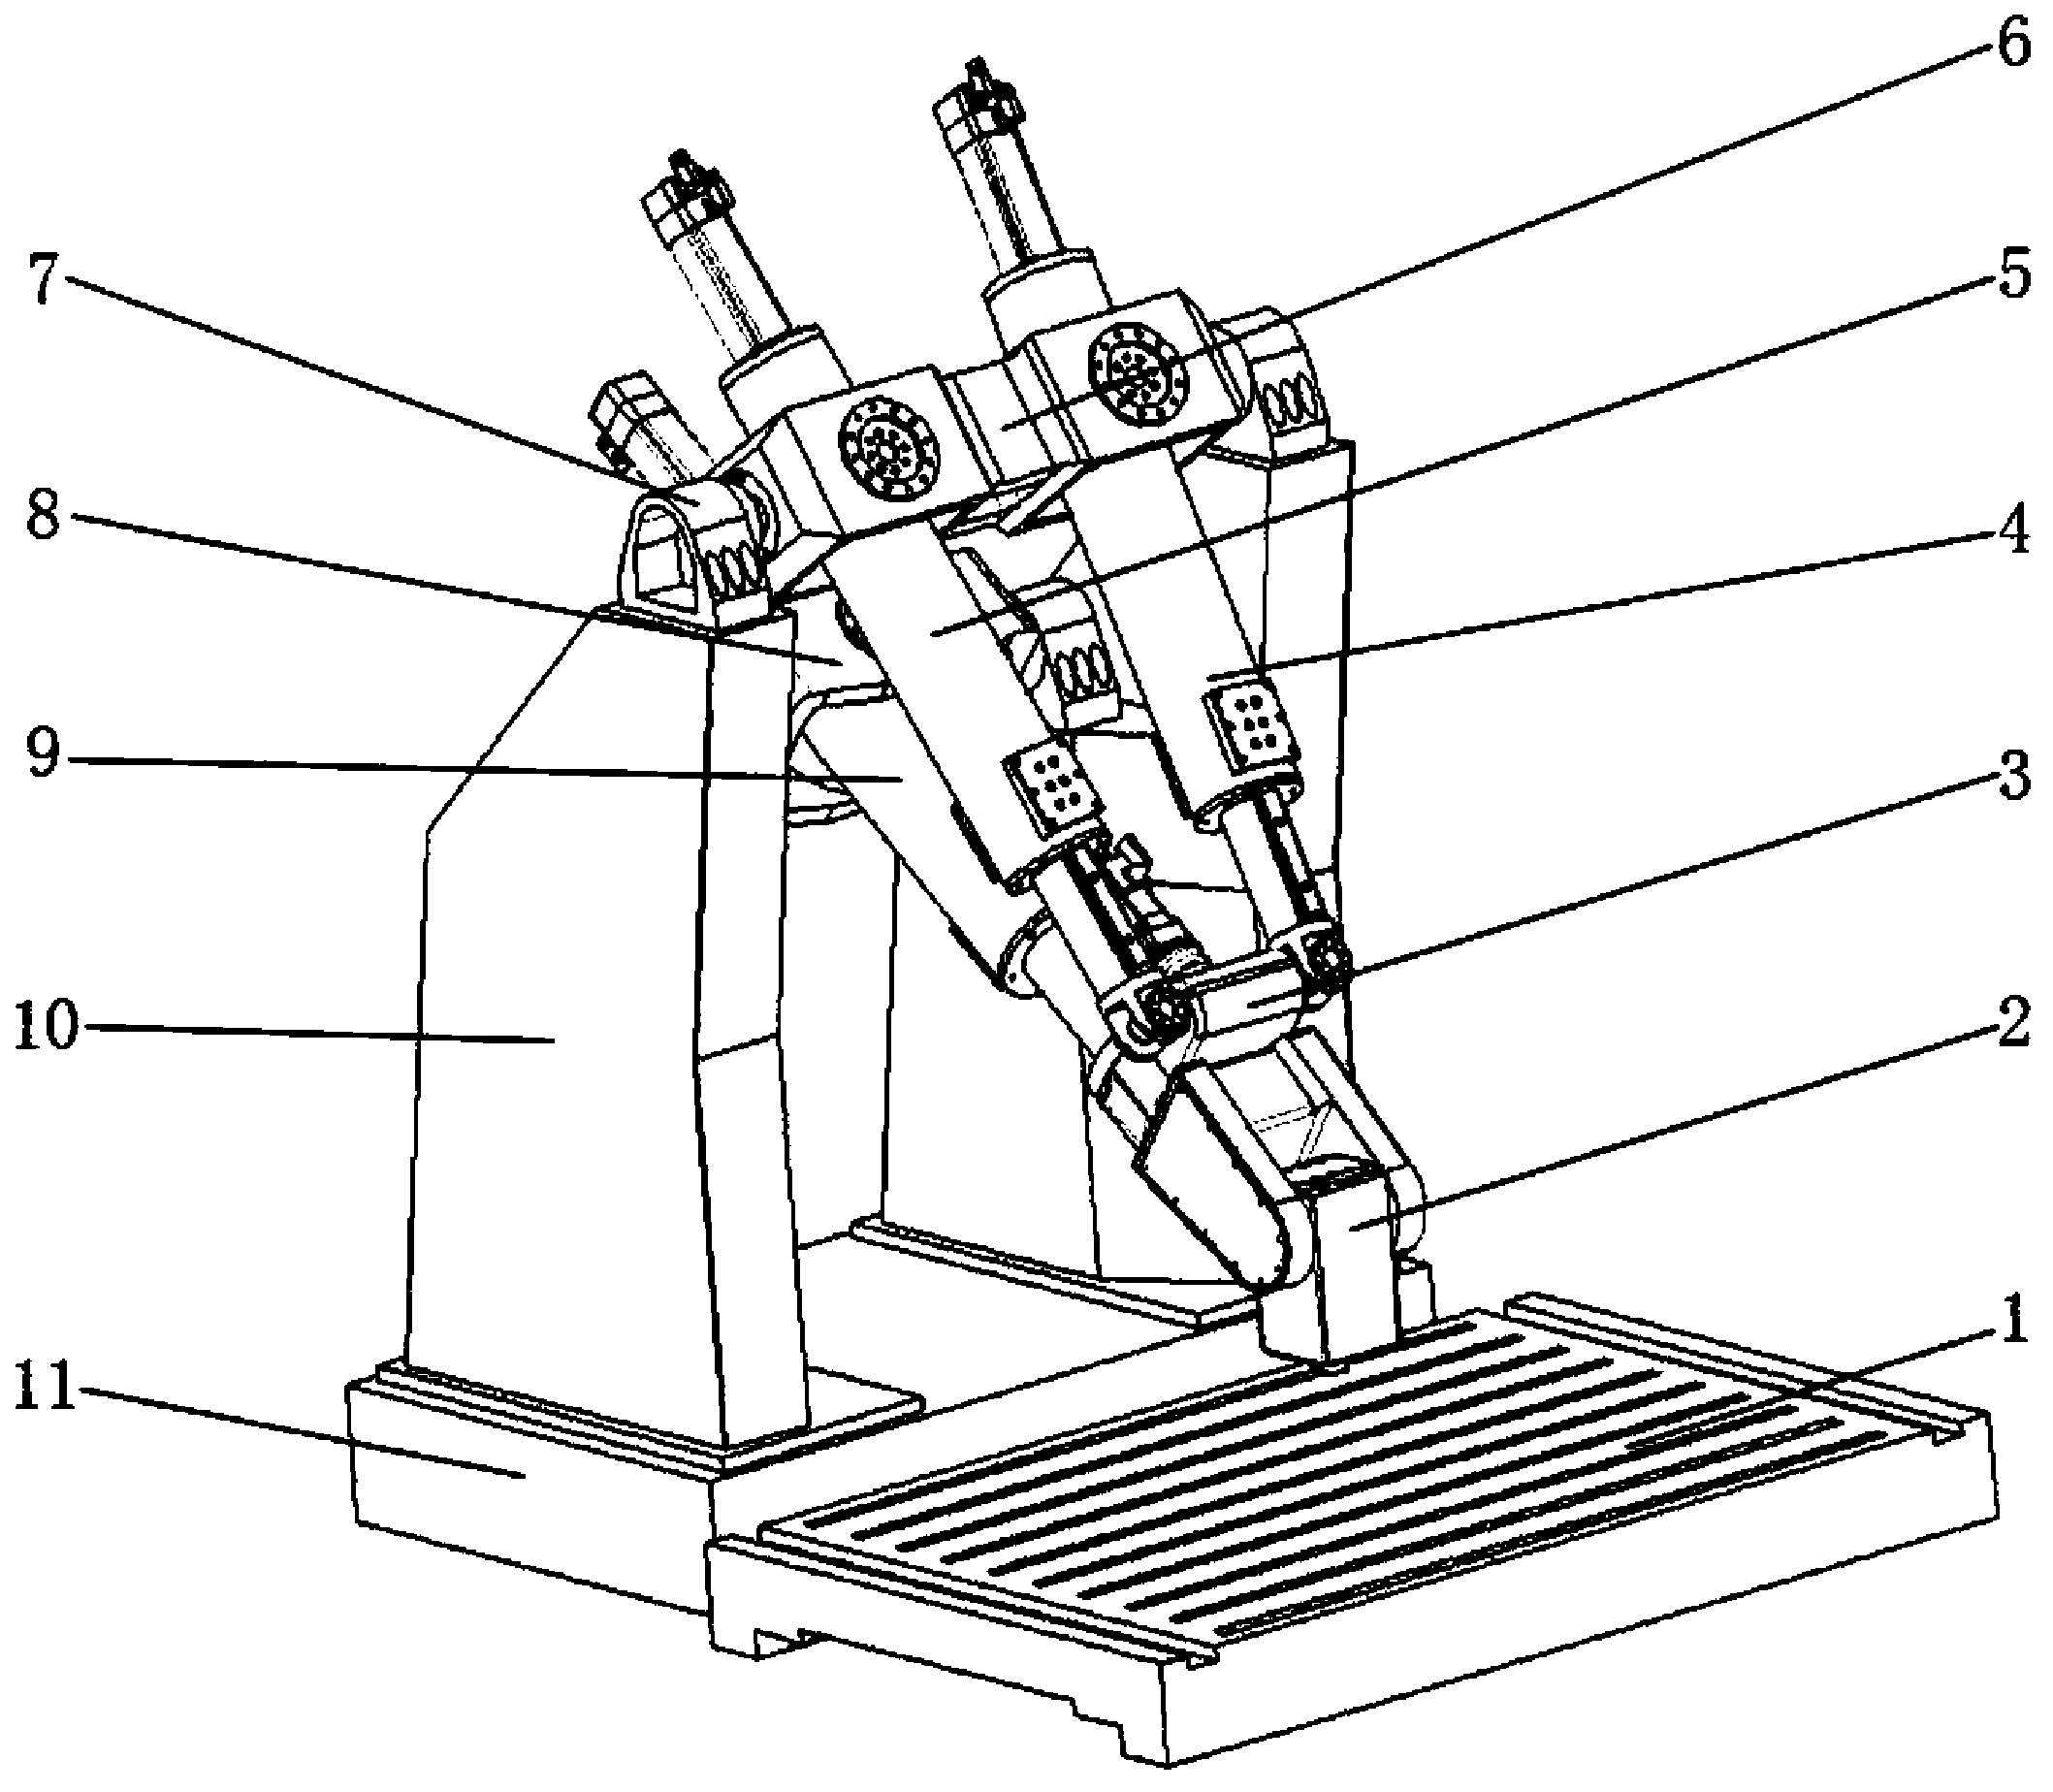
\includegraphics[width = 0.5\textwidth]{Cap2_DisenoEspecificaciones/Figura/WO2019091425A1.pdf}
    \caption{Robot de 5-GDL conexión hibrida}{Fuente:\citep{patent:WO2019091425A1}}
    \label{fig:WO2019091425A1}
\end{figure}

\textbf{CN109091233A} - \textit{Puncturing operation robot based on series and parallel structure} \citep{patent:CN109091233A}: Esta patente pertenece al campo técnica de los dispositivos médicos, es un robot para cirugía de punción basado en una estructura en serie-paralela. La máquina está compuesta de una base, un mecanismo de ajuste y postura y un mecanismo de inserción de aguja. Las acciones del robot de cirugía de punción del control atreves de los cinco grados de libertad de la estructura serie- paralela.

\textbf{ES2433664T3} - \textit{Dispositivo guiador dirigible} \citep{patent:ES2433664T3}: Esta patente presenta una sonda robótica articulada, con 2 mecanismo que pueden operar coordinados o según la configuración que se necesite, flácido o rígido.

\textbf{US5715729A} - \textit{Machine tool having parallel structure} \citep{patent:US5715729A}: Trata del diseño de un robot paralelo con seis grados de libertad, Figura \ref{fig:US5715729A}, con 6 brazos y 6 motores, una placa base fija y una sección móvil, destinado a trabajar materiales duros y a un enfoque industrial.

\begin{figure}[ht]
    \centering
    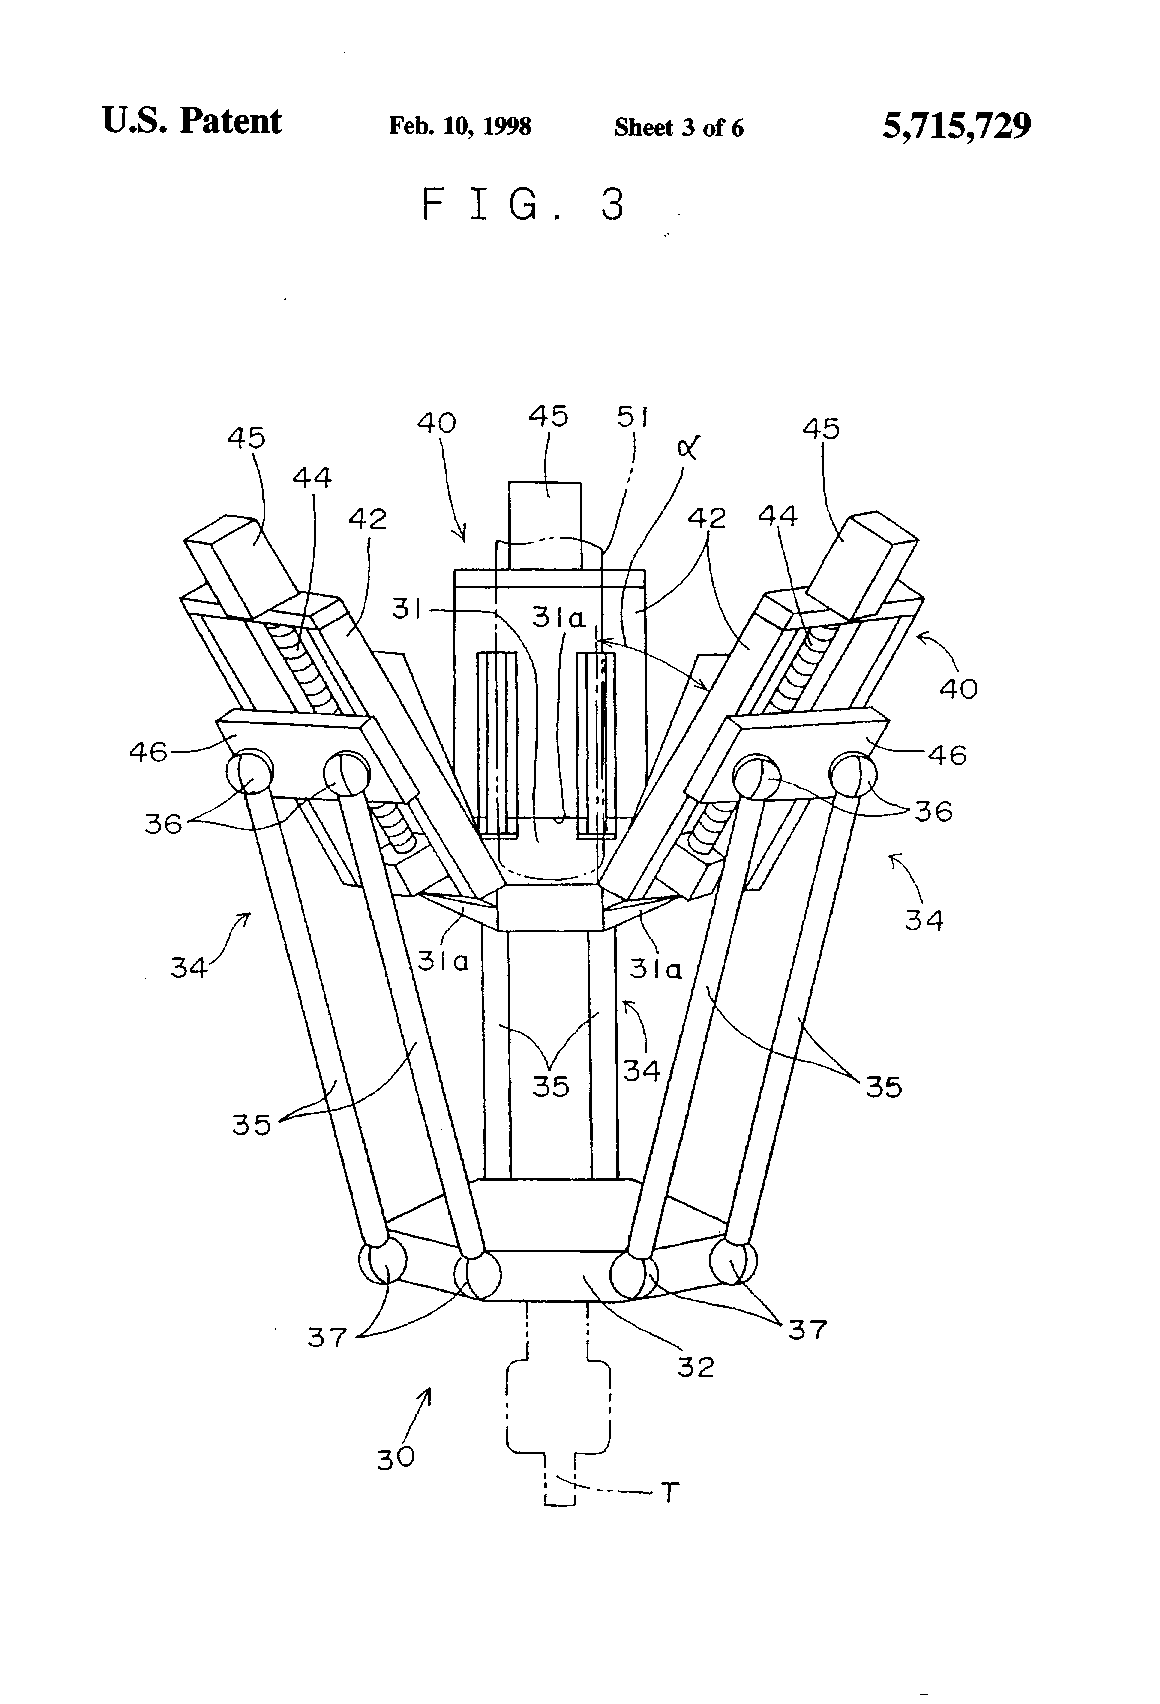
\includegraphics[width = 0.5\textwidth ]{Cap2_DisenoEspecificaciones/Figura/US5715729A.pdf}
    \caption{Estructura para máquina paralela}{Fuente:\citep{patent:US5715729A}}
    \label{fig:US5715729A}
\end{figure}

\textbf{ES2392059B2} - \textit{Robot de estructura cinemática híbrida para el guiado de la inserción de agujas, catéteres y elementos quirúrgicos para procedimientos de cirugía mínimamente invasiva.} \citep{patent:ES2392059B2}: 

\textbf{CN109348795A} - \textit{A kind of replanting system and its implementation based on parallel robot} \citep{patent:CN109348795A}: La invención describe con un sistema de transporte basado en un robot paralelo y un método de implementación del sistema. EL sistema está compuesto por Una estructura de marco, robot paralelo y un dispositivo de transporte.

\textbf{US8776632B2} - \textit{Actuación de baja carrera para un robot en serie.} \citep{patent:US8776632B2}: Esta patente fue financiada por el gobierno de USA, específicamente la NASA se refiere al control de movimiento y Diseño de empaque de un dedo tendón y otra articulaciones


%\textbf{CN201579788U} - \textit{Opened field type six-freedom-degree serial-parallel processing robot}: La patente es de un robot serie-paralelo de seis grados de libertad (campo abierto) que cuenta con sensores de fuerza, cámara de visión que envían información a un controlador que calcula donde está el husillo y la fuerza para moverlo.
\newpage
\definecolor{Gray}{gray}{0.85}
\begin{longtable}{|>{\columncolor[gray]{0.85}}p{0.25\textwidth}|p{0.4\textwidth}|p{0.33\textwidth}|}
\hline \rowcolor{Gray} 
\textbf{\large Patente} & \textbf{\large Ventajas} & \textbf{\large Desventajas} \\ \hline \endhead
CN109676587A & Fuerzas de fricción pequeñas entre los accesorios. & \\
 & Se puede ajustar el coeficiente de amplificación de ángulo. & Volumen de la máquina. \\
 & Cadenas de ramificación simples. & \\ \cline{1-3}
 
ES2588015 & Gran espacio de trabajo, & Baja compacticidad \\
 & logra realizar geometrias muy complejas. & ,Necesita una base giratoria. \\ \cline{1-3}
 
WO2019091425A1 & Una mejora en la rigidez integral de la estructura. & \\
 & Reducción en la dificultad de control. & \\
 & Análisis cinemático es simple y respuesta dinámica buena. & \\
 & Por la combinación de cabezal oscilante de dos grados de libre la plataforma móvil, se amplía el espacio de trabajo de una máquina de herramienta. & \\ \cline{1-3}
 
ES2392059B2 & Mecanismo hibrido, Diseño modular, 6 grados de libertad, Sistema hibrido, bajo peso, cuenta con un sistema guiado por laser. & Sistema de control complejo, estructura ligeramente debil.\\
 & . & \\ \cline{1-3}
 
CN109091233A & La operación de ajuste y postura de la aguja se pueden completar automáticamente. & Un tamaño pequeño conveniente para el uso médico, pero no para el uso industrial \\
 & Una estructura simple en general. &  \\ \cline{1-3}

ES2433664T3 & Puede ser utilizado en multiples campos por su adaptibilidad. Se pueden adaptar camaras, medicamentos entre otros al interior del dispositivo, es muy flesible. Ideal para espacios reducidos (Tuberias). & Solo maneja 3 ejes, maneja bajas cargas, se necesitan una gran cantidad de sensores y controladores para operar correctamente. Se hace necesario la sincronizacion del mecanismo interno con el externo.
  \\ \cline{1-3}

US5715729A & Trabajo con grandes cargas, sistema de control "sencillo" & \\ \cline{1-3}

ES2392059B2 &  grados de libertad, Sistema hibrido, bajo peso, cuenta con un sistema guiado por laser, cuenta con un sistema modular el cual permite cambiar facilmente de herramienta, alta precisión.
 & Sistema de control complejo, estructura levemente debil.  \\ \cline{1-3}

AU2007297702B2 & Altamente preciso, portable, cuenta con herrramientas modulares. & Espacio de trabajo reducido, se debe de tener en cuenta las posibles singularidades, en funcion de su area de trabajo, es poco compacto.\\ \cline{1-3}


CN109348795A & Mejora de la eficiencia enormemente. & \\
 & El sistema es más liviano. & \\
 & Una estructura simple y es más conveniente para la operación en comparación de un robot serie. & \\ \cline{1-3}
 
%CN201579788U & Compacta & \\
% & Económica & \\
% & Alta Precisión & \\ \cline{1-3}
\caption{Revisión de Patentes}{Fuente: Elaboración Propía}
\label{table:PatentRevision}
\end{longtable}
%\newpage
%%%%%   Definición de Especificaciones    %%%%%
\section{Definición de Especificaciones}
\subsection{Despliegue de Función de Calidad (QFD)}

La matriz QFD es una parte fundamental del proceso de diseño que facilita la generación de especificaciones de el producto o maquina a fabricar, permite hacer una comparación entre las caracteristicas que intervienen en este teniendo en consideracion los requerimientos del cliente y de diseño. La matriz QFD presenta de manera resuminda y confronta las caracteristicas requeridas, los pros y contras, de manera que se traduzcan tales requerimientos en variables de ingenieria (medibles) y de este modo facilitar la toma de desciciones y la propuesta de alternativas.

\begin{landscape}
\begin{figure}[hb!]
    \centering
    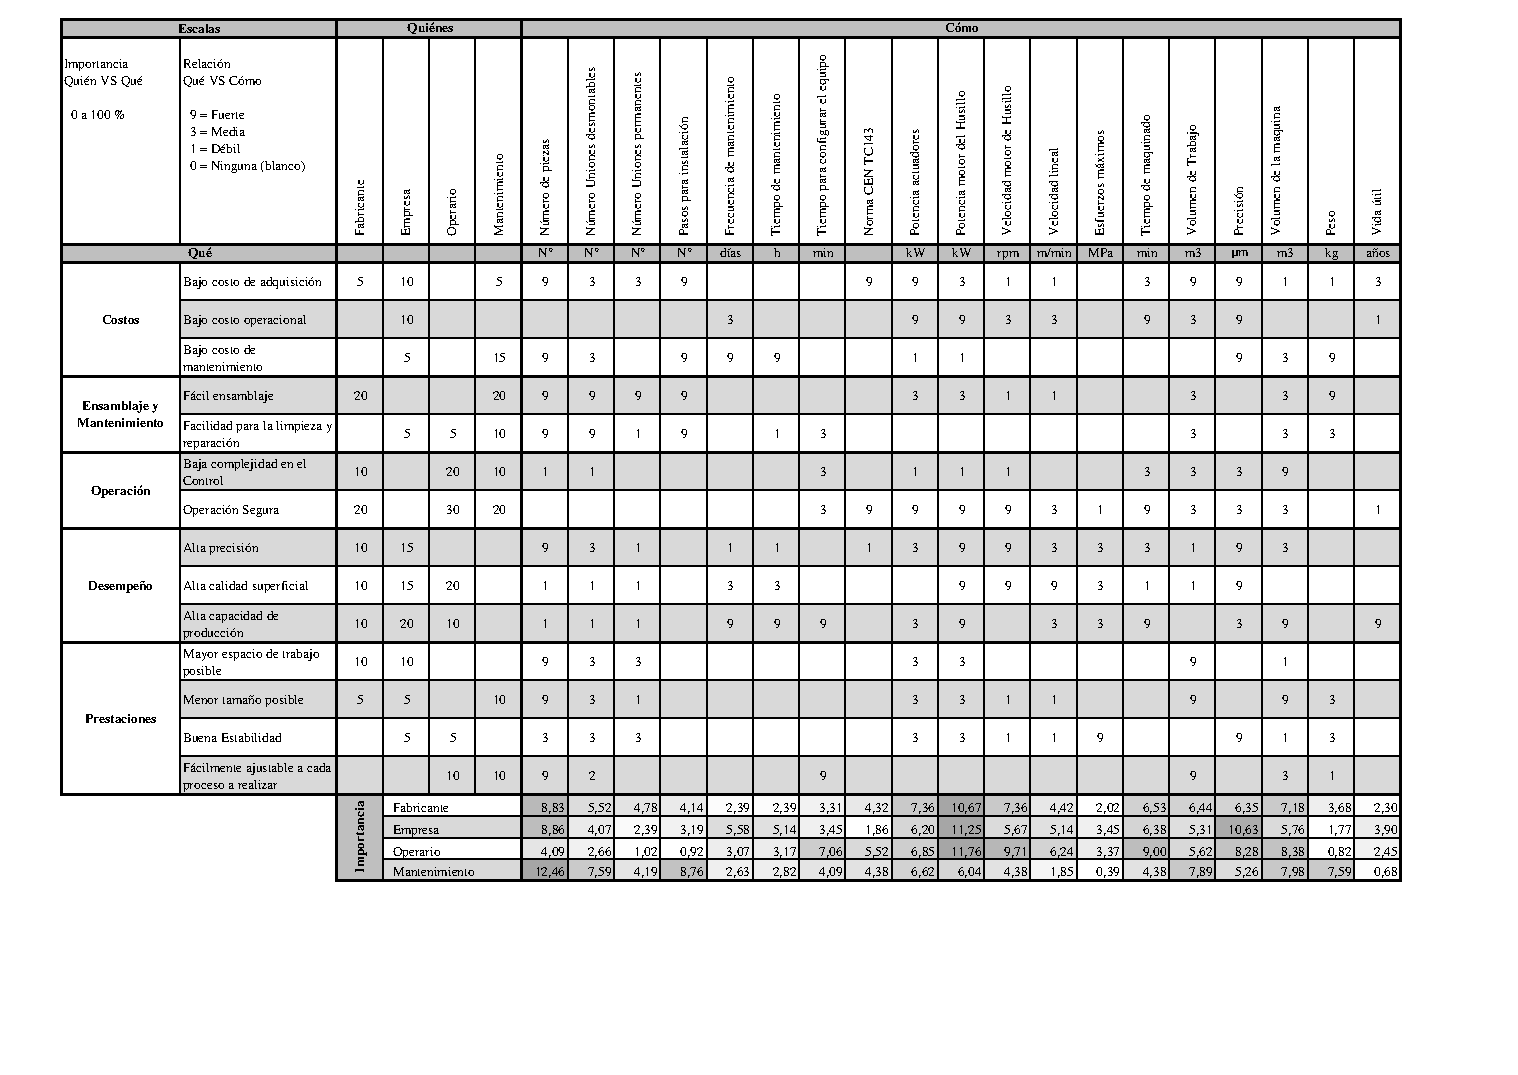
\includegraphics[scale=0.9]{Cap2_DisenoEspecificaciones/Figura/QFD.pdf}
    \caption{QFD}
    \label{fig:QFD}
\end{figure}
\end{landscape}

\subsection{Listado de referencia de especificaciones}

La lista de referencia es una estrategia de diseño que busca desarrollar una lista de especificaciones iniciales suficientes, las cuales se construyen a partir de los estudios del estado del arte, estado de la tecnica y analisis del QFD donde se intenten abordar todos los aspectos y elementos del diseño y apuntar a la obtencion de especificaciones completas. 
\begin{longtable}{|>{\columncolor[gray]{0.85}}p{0.25\textwidth}|p{0.70\textwidth}|}
    \cline{1-2} \rowcolor[gray]{0.85}
    \textbf{Concepto} & \textbf{Determinaciones } \\ \hline \endhead
    Funcion     & Descripcion de las funciones principales, ocasionales y accidentales del producto.\\ \cline{1-2}
    Dimensión   & Espacios, Volumenes, masas, longitudes, alturas, anchuras, diametros; numero y disposicion de elementos \\ \cline{1-2}
    Movimientos & Tipos de movimiento; desplazamientos, secuencias y tiempos; trayectorias, velocidades y aceleraciones.\\ \cline{1-2}
    Fuerzas     & Magnitud, direccion y sentido de fuerzas y momentos; variacion en el tiempo; desequilibrios y deformaciones admisibles.\\ \cline{1-2}
    Energia     & Accionamientos mecanico y otros conversores de energia: alimentacion y control; transmisiones; potencia y rendimiento.\\ \cline{1-2}
    Materiales  & Flujo, transporte y transformacion de materiales; limitaciones o preferencias sobre su uso; condicionantes de mercado.\\ \cline{1-2}
    Señales y control & Señales de entrada y salida; sensores y actuadores; funciones del sistema de control.\\ \cline{1-2}
    Fabricacion y montaje & Volumen previsto de produccion y cadencia en el tiempo; limitaciones o preferencias en procesos y equipamientos; variantes en el producto de flexibilidad en la fabricacion.\\ \cline{1-2}
    Transporte y distribucion & Embalaje y transporte: dimensiones, masas, orientacion, golpes; instalacion, montaje y puesta a punto.\\ \cline{1-2}
    Vida util y Mantenimiento & Vida prevista; fiabilidad y mantenibilidad; tipo de mantenimiento e intervalos de servicio; criterios sobre recambios.\\ \cline{1-2}
    Costes y plazos & Costes de desarrollo y preparacion de utillaje; plazos de desarrollo y tiempo para el mercado.\\ \cline{1-2}
    Seguridad y ergonomía & Sistemas y dispositivos de seguridad; relacion con el usuario; operacion, inteligibilidad, confort y aspecto.\\ \cline{1-2}
    Impacto ambiental & Consumos de energía y materiales; limitaciones al impacto ambiental en la fabricacion, utilizacion y fin de vida.\\ \cline{1-2}
    Apectos legales & Cumplimiento de noremativas (Funcion de los usos y mercados); evitar la colision con patentes.\\ \cline{1-2}
    
    
    \caption{Lista de referencia de especificaciones}{Fuente: \cite{Riba2002}}
\end{longtable}
~
La tabla mostrada es el modelo de lista de referencia del método MEPEIS y se utilizó para la construcción del listado de referencia propio.
\begin{longtable}{|>{\columncolor[gray]{0.85}}p{0.25\textwidth}|c|p{0.60\textwidth}|}
    \cline{1-3} \rowcolor[gray]{0.85}
    \textbf{Concepto} & \textbf{R/D} & \textbf{Descripcion } \\ \hline %\endhead
    Función     & R & Realizar operaciones de Fresado y Taladrado \\ \cline{1-3}
    Dimensión   & R & Relación Espacio de Trabajo/Volumen de la Máquina superior a $1,3\%$ \\
                & D & Espacio de Trabajo superior a $500\times 500\times 500$ mm \\ \cline{1-3}
    Movimientos & D & Entradas  paralelas \\
                & R & Presicion de 0.005 mm \\ \cline{1-3}
    Fuerzas     & R & Disminución de par requerido \\ \cline{1-3}
    Energía     & R & Ahorro Energético de los motores \\ \cline{1-3}
    Materiales  & R & Rigidez (Vibraciones) \\
                & R & Resistencia a Fatiga \\ \cline{1-3}
    Señales y Control   & R & RPM \\
                        & R & Velocidad de avance \\
                        & D & Aceleraciones \\
                        & R & Posición \\
                        & D & Torque \\ \cline{1-3}
    Vida Útil y Mantenimiento & D & Vida útil mayor a 10 años \\ \cline{1-3}
    Fabricación y Montaje   & D & Fabricación con piezas estándares y montaje modular \\
                            & D & Fácil remplazo de piezas dañadas, sea por la facilidad de comercialización (piezas estándar) o la capacidad de fabricar las mismas \\
                            & D & Facil mantenimiento por diseño moludar\\ \cline{1-3}
    Costos de Fabricación   & D & Costos de Fabricación inferiores a 40 Millones de pesos \\ \cline{1-3}
    Seguridad               & R & Alta protecion al operario \\
                            & R & Protecciones Electricas y Termicas de la maquina \\
    \cline{1-3}
    \caption{Requerimientos para Máquina CNC de 3 ejes}{Fuente: Elaboración propia}
\end{longtable}

\section{Normas}
\begin{center}
    \begin{longtable}{|>{\columncolor[gray]{0.85}} p{0.2\textwidth}| p{0.2\textwidth}| p{0.5\textwidth}| }
    \rowcolor[gray]{0.85} \hline
    \textbf{Estandar} & \textbf{Norma} & \textbf{Titulo}  \\ \hline \endhead
        {CEN} & TC 143      & Standardization in the field of safety of machine tools, their accessories and tools designed to form and to machine cold metal both with and without the removal of metal. \\ \hline
        {ISO} & 230-2       & Determination of accuracy and repeatability of positioning of numerically controlled axes. \\ \hline
        {ISO} & TR 230-8    & Test code for machine tools-Vibrations. \\ \hline
        {ISO} & 3685        & Tool-life testing with single-point turning tools. \\ \hline
        {ISO} & 1985        & Machine tools-Test conditions for surface grinding machines with vertical grinding wheel spindle and reciprocating table-Testing of accuracy.\\ \hline
        {ISO} & 230-3       & Determination of thermal effects. \\ \hline
        {ISO} & 8373       & Manipulating industrial robots.\\ \hline
        {ISO} & 9409-2       & Manipulación de robots industriales. Interfaces mecánicas. Parte 2: Ejes.\\ \hline
        
        \caption{Normas a utilizar}{Fuente: Elaboración Propia}
        \label{table:Normas}
       \end{longtable}
\end{center}